%**********************************************************************%
%* Physics for Poets Learning Notes
%* 4th edition
%* Author: Robert March
%* Chapter: 12
%* Notes: camilo tejeiro
%**********************************************************************%

% article type 12 pt font.
\documentclass[12pt, letterpaper]{article}

%----------------------- External Packages ----------------------------%
% package to insert images to our doc.
\usepackage{graphicx}

%------------------ Dimensions and Page Layout--------------------------%

%----------------------- LaTeX Environments ---------------------------%

%------------------------- LaTeX Commands -----------------------------%

%------------------------- Document Content ---------------------------%
% make title built in command values
\title{Chapter 12, Did God Have Any Choice?}
\author{Learning Notes, Physics for Poets}
\date{}

\begin{document}

    \maketitle

    \section{The Principle of Equivalence}
    To develop his theory of gravity, which he called general relativity, 
    Einstein added one more postulate to the theory of relativity, mainly:
    
    \textit{No experiment performed in one place can distinguish a gravitational 
    field from an accelerated reference frame}.
    
    The words in ``one place'' are important. Einstein did not eliminate all 
    distinctions between gravity and accelerated reference frames. If we 
    compare the fall of objects in different places on Earth, we will find 
    that they all head toward the Earth's center. No accelerated reference 
    frame can duplicate that pattern.
    
    What Einstein is saying is simply that all objects respond to a gravitational 
    field in the same way they respond to being in an accelerated frame.
    
    We can see this more graphically through the following examples:
 
    \begin{figure}[h!]
        \caption{A person inside an accelerating rocket}
        \centering
        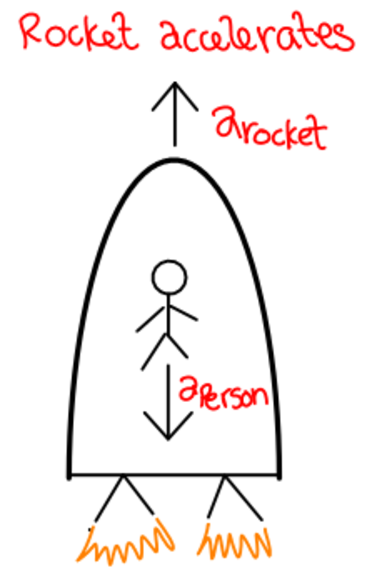
\includegraphics[scale=0.5]{rocket_accelerates_person.pdf}
    \end{figure}       
    
    As the rocket accelerates the person feels as if he is pulled 
    down to floor (the floor is pushing against his feet); to him it feels 
    just as if he is subject to the force of gravity. 
    
    But this equivalence effect also works on light (as it should since we know 
    energy is equivalent to mass). The following example shows how the path 
    of light is curved in an accelerated frame.
  
    \begin{figure}[h!]
        \caption{A laser inside an accelerating rocket}
        \centering
        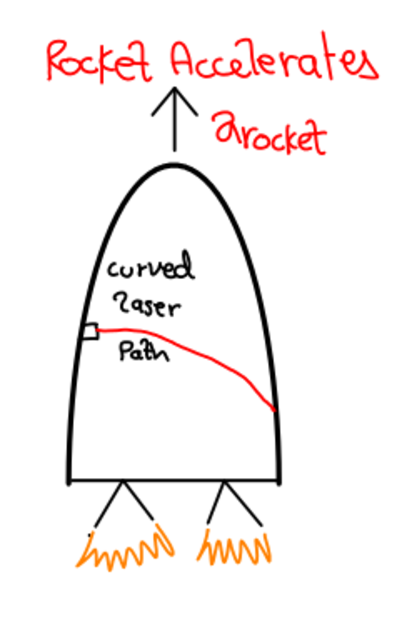
\includegraphics[scale=0.5]{rocket_accelerates_light.pdf}
    \end{figure}  
    
    As you can see the laser beam curves down (the rocket moves up while 
    the light is traveling) and the same effect will happen in a 
    gravitational field.
 
     \begin{figure}[h!]
        \caption{Light affected by a gravitational field}
        \centering
        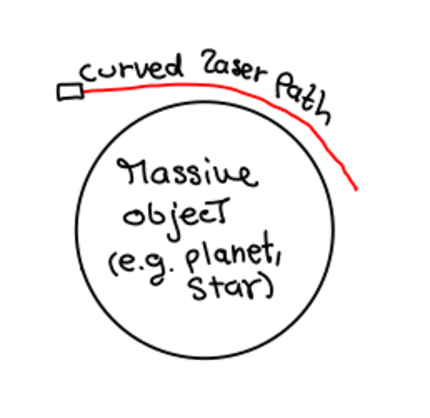
\includegraphics[scale=0.5]{planet_curves_light.pdf}
    \end{figure}    
    
    Einstein's conclusion was that there is absolutely no need 
    for a ``force'' of gravity as long as space and time are curved.
    
    However, it is hard to imagine what curved space-time actually means, 
    it's almost like trying to figure out whether the earth is round by 
    looking at a map. But, let's go over a couple of examples and see if 
    our imagination can help us visualize these concepts. 
    
    \subsection*{What is Curved Space?}
    To visualize curved space it is helpful to think of the planets in our 
    solar system as if they are all sitting on a thin flat fabric, and 
    because the planets have mass, they stretch down the fabric. The 
    following illustration helps convey the image.
    
     \begin{figure}[h!]
        \caption{The stretch of the space fabric}
        \centering
        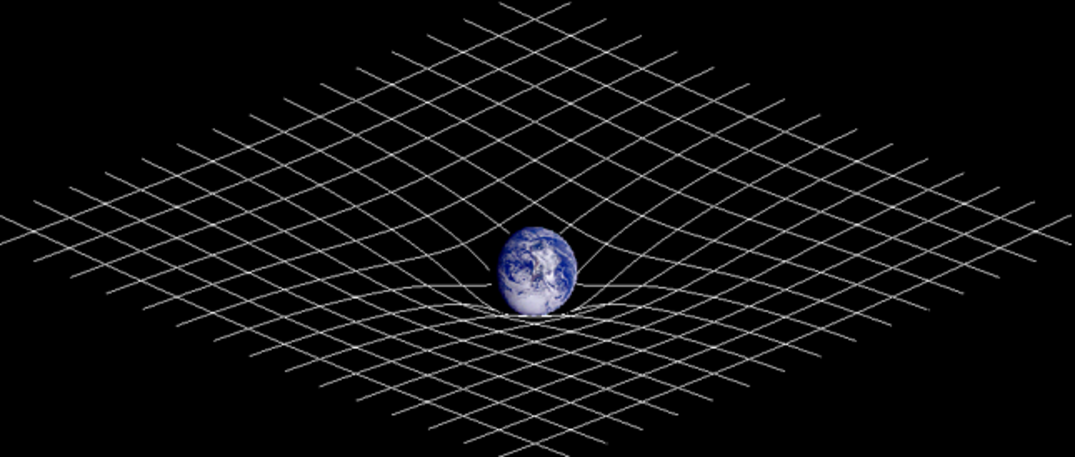
\includegraphics[scale=0.5]{space_time_curvature.pdf}
    \end{figure}      
    
    \emph{But how does a curved space account for the effect of gravity?} 
    It does so by affecting the path of objects as they coast along on 
    top of the fabric, the results is a type of motion akin to objects subject 
    to the force of gravity.
    
    \medskip
    So, instead of talking about a force of attraction, 
    we can say that the object ``rolled down the curved space fabric''. 
    But, we can also see that the fabric stretches more as we place 
    more massive objects on it, this is akin to the mass force relationship 
    of gravity.
    
    \medskip
    Let's take another example: We previously saw the accelerating rocket 
    and the curved path of light. But, we can also see a similar effect 
    if we look at the path of light (x going into the page) as it rolls 
    down in a curved space fabric. 
    
     \begin{figure}[h!]
        \caption{The Laser rolls down the curved space fabric}
        \centering
        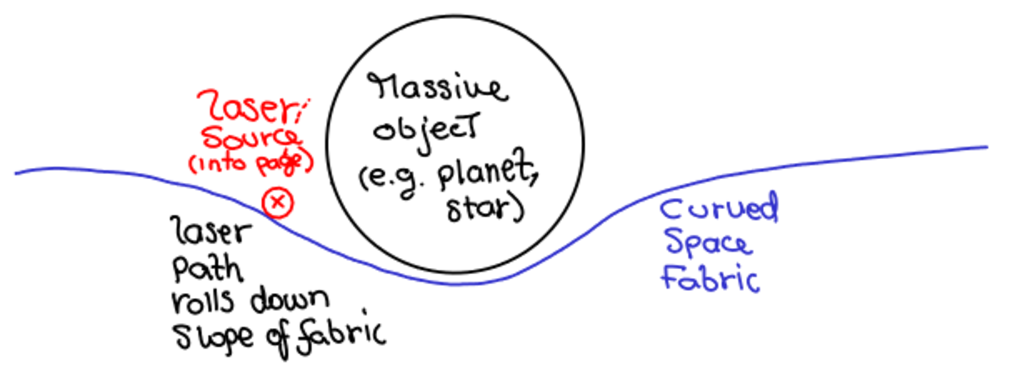
\includegraphics[scale=0.5]{planet_curves_space_fabric.pdf}
    \end{figure}         
    
    \subsection*{What is Curved Time?}
    Curved time is concept which can be a little bit more abstract, mainly 
    because we are used to taking time as a constant (e.g. an hour is an 
    hour anywhere) but it simply means that time is also affected by the 
    geometry of the space-time fabric.
    
    \medskip
    the following example helps convey this concept:
     \begin{figure}[h!]
        \caption{Clocks in an accelerated frame}
        \centering
        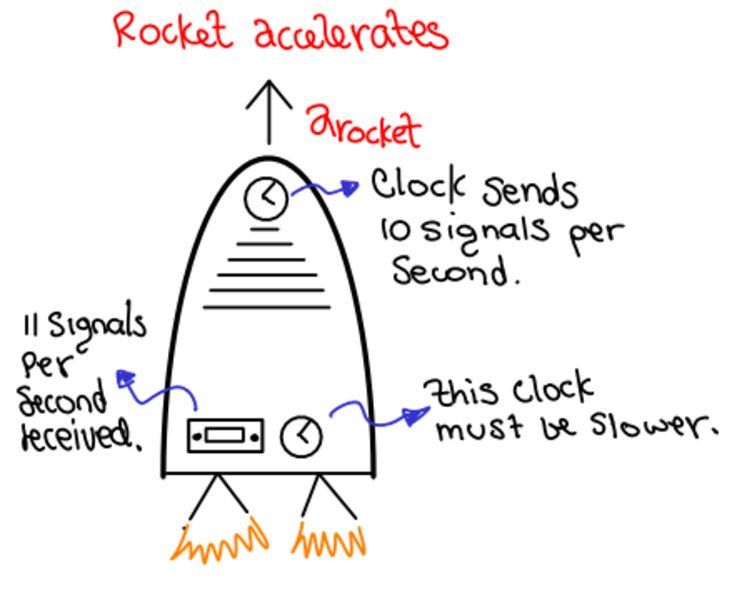
\includegraphics[scale=0.5]{rocket_accelerates_clock.pdf}
    \end{figure}      
    
    The rocket is accelerating, so while the top clock is putting out signals 
    at a constant rate (10 signals per second), the bottom of the rocket 
    is accelerating, and the detector is receiving more signals per second
    (11 signals per second). Thus, the bottom clock must be running slower, 
    and the same effect must(and does) happen in a gravitational field.
    
    \medskip
    So, general relativity tells us that clocks closer to a massive object 
    (stronger gravitational field) run slower and those farther away run 
    faster (weaker gravitational field). Here is a visual picture.

     \begin{figure}[h!]
        \caption{Clocks in a gravitational field}
        \centering
        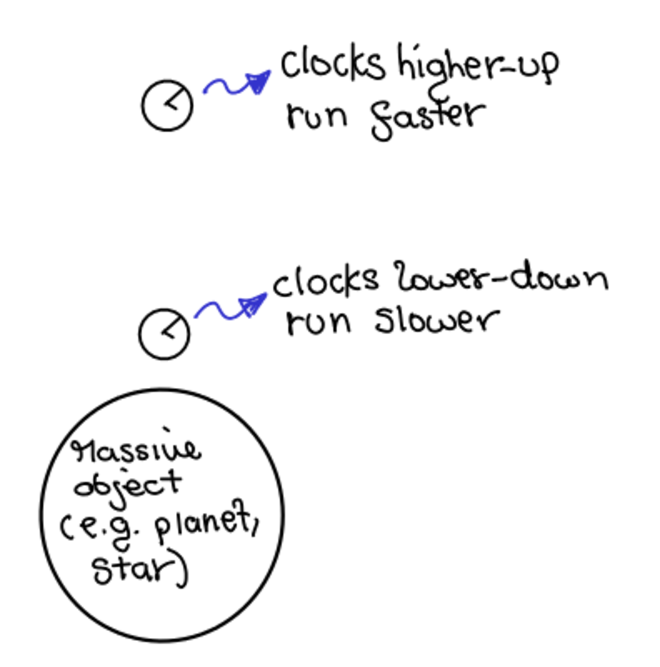
\includegraphics[scale=0.3]{planet_slows_clocks.pdf}
    \end{figure} 
    
    \subsection*{Curved space-time the complete picture}
    Our complete picture now involves a reality where mass curves the fabric 
    of space and time. This effect not only accounts for the mechanics and 
    interactions of large objects which we previously accounted for through 
    the use of gravity, but it introduces a new concept, time is no longer 
    a constant. 
    
    I leave you with the following picture.
    
    \begin{figure}[h!]
        \caption{Clocks in a gravitational field}
        \centering
        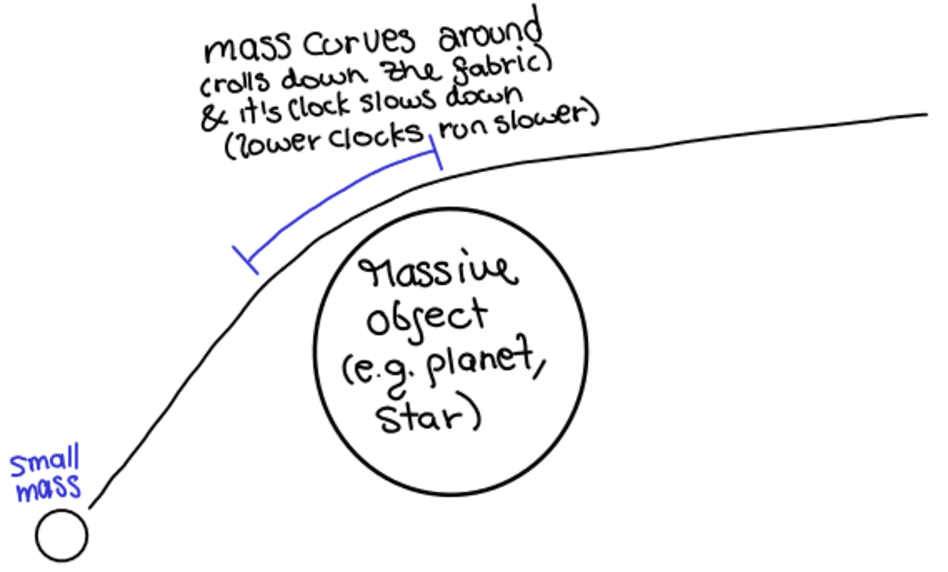
\includegraphics[scale=0.5]{planet_curves_space_time.pdf}
    \end{figure}    
    
    As the mass passes close to the large planet it rolls down the stretched 
    space fabric and curves around the planet, it's clock also slows down.
    
\end{document}

